%% This is file `tlsflyleaf-fr.tex',
%% Copyright 2013 Tristan GREGOIRE
%
% This work may be distributed and/or modified under the
% conditions of the LaTeX Project Public License, either version 1.3
% of this license or (at your option) any later version.
% The latest version of this license is in
%   http://www.latex-project.org/lppl.txt
% and version 1.3 or later is part of all distributions of LaTeX
% version 2005/12/01 or later.
%
%
% This work has the LPPL maintenance status `maintained'.
% 
% The Current Maintainer of this work is T. GREGOIRE
%

\documentclass{scrartcl}

% ============================================================
% PACKAGE
\usepackage{fixltx2e}
\usepackage{etex}
\usepackage{lmodern}
\usepackage[T1]{fontenc}
\usepackage[utf8]{inputenc}
\usepackage{textcomp}
\usepackage{microtype}
\usepackage{hyperref}
\usepackage{listings}
\usepackage{color}
\usepackage{graphicx}
\usepackage[toc]{multitoc}
\usepackage{tocloft}
\usepackage{wasysym}

\hypersetup{linktocpage,
    colorlinks,
    citecolor=blue,
    filecolor=blue,
    linkcolor=blue,
    urlcolor=blue
}

\definecolor{dkgreen}{rgb}{0,0.6,0}
\definecolor{gray}{rgb}{0.5,0.5,0.5}
\definecolor{mauve}{rgb}{0.58,0,0.82}

\lstset{language=tex,
    tabsize=2,
    showstringspaces=false,
    basicstyle={\small\ttfamily},
    numbers=left,
    numberstyle=\tiny\color{gray},
    keywordstyle=\color{blue},
    commentstyle=\color{dkgreen},
    breaklines=true,
    breakatwhitespace=true,
    title=\lstname,
    escapeinside={\%*}{*)},
    frame=single
}


% ============================================================
% COMMAND
\newcommand*{\mail}[1]{\href{mailto:#1}{\texttt{#1}}}
\newcommand*{\www}[2]{\href{#2}{\texttt{#1}}}
\newcommand*{\pkg}[1]{\textsf{#1}}
\newcommand*{\cs}[1]{\texttt{\textbackslash#1}}
\makeatletter
\newcommand*{\cmd}[1]{\cs{\expandafter\@gobble\string#1}}
\makeatother
\newcommand*{\meta}[1]{\textlangle\textsl{#1}\textrangle}
\newcommand*{\marg}[1]{\texttt{\{}\meta{#1}\texttt{\}}}
\newcommand*{\opt}[1]{\texttt{#1}}
\newcommand*{\cmdarg}[1]{\{<\textit{#1}>\}}
\newcommand*{\file}[1]{\textit{\texttt{#1}}}

\addtokomafont{title}{\rmfamily}

% ============================================================
% TITLE
\title{Le paquet\thanks{Ce manuel correspond \`a \pkg{tlsflyleaf.sty}~v1.1, dat\'e du 22 Mars 2013.} \ \pkg{tlsflyleaf}}
\author{Tristan GR\'EGOIRE\thanks{\mail{tlsflyleaf@onada.fr}}}
\date{22 Mars 2013}

% ============================================================
% DOCUMENT
\begin{document}
\maketitle

\begin{abstract}
	\noindent
    Ce paquet fourni une liste de commandes, d'utilisation simple, qui permettent
    de cr\'eer une page de garde pour le manuscrit de th\`ese.
\end{abstract}

\renewcommand{\cftsecleader}{\cftdotfill{\cftdotsep}}
\setlength\columnseprule{1pt}
\renewcommand\contentsname{\begin{center}\hrulefill \hspace*{1cm} Sommaire\hspace*{1cm} \hrulefill\end{center}}
\tableofcontents
~
\hrule


%%%%%%%%%%%%%%%%%%%%%%
\section{Introduction}
%%%%%%%%%%%%%%%%%%%%%%
Ce paquet fourni un moyen simple pour cr\'eer et personaliser la page de garde officielle de l'\textit{Universit\'e de Toulouse III}.
Il aidera de nombreux doctorants lors de la r\'edaction de leur th\`ese
en leur permettant de reproduire \`a l'aide de commandes simples la page de garde officielle fourni
dans un format propri\'etaire et non utilisable en \LaTeX.

L'usage principal est similaire \`a celui de la commande \cmd{\maketitle} avec des commandes \`a d\'eclarer dans le
pr\'eambule du document \LaTeX{} et une seule commande (\cmd{\makeflyleaf}) \`a utiliser dans le corps
du document.

%%%%%%%%%%%%%%%%%%%%%%
\section{Dépendances}
%%%%%%%%%%%%%%%%%%%%%%
\begin{enumerate}
    \item[\LaTeX{}] une version r\'ecente de \LaTeXe ($\ge$ 2011)
    \item[\pkg{eso-pic}] une version récente de \pkg{eso-pic.sty}\\
      \www{http://www.ctan.org/tex-archive/macros/latex/contrib/eso-pic}{http://www.ctan.org/tex-archive/macros/latex/contrib/eso-pic}
    \item[\pkg{geometry}] une version récente de \pkg{geometry.sty}, il faut une version $\ge$ 5.\\
      \www{http://www.ctan.org/tex-archive/macros/latex/contrib/geometry}{http://www.ctan.org/tex-archive/macros/latex/contrib/geometry}
	  \item[\pkg{shadowtext}] paquet : \pkg{shadowtext.sty}~v0.3, dat\'e du 2012/05/07 \\
	    \www{http://www.ctan.org/tex-archive/macros/latex/contrib/shadowtext}{http://www.ctan.org/tex-archive/macros/latex/contrib/shadowtext}
\end{enumerate}

%%%%%%%%%%%%%%%%%%%%%%
\section{Pr\'eambule}
%%%%%%%%%%%%%%%%%%%%%%
On charge le paquet \`a l'aide de la commande :
\cmd{\usepackage[\textit{<option>}]\{tlsflyleaf\}}

Il est aussi n\'ecessaire de d\'efinir les informations que doit contenir la page de garde.
Pour cela le paquet fourni les commandes suivantes :
\begin{description}
    \renewcommand{\makelabel}[1]{#1}
	\item[\cmd{\FRtitle}\cmdarg{titre}] Version fran\c{c}aise du titre de la th\`ese.
	\item[\cmd{\defencedate}\cmdarg{date}] date de la soutenance.
	\item[\cmd{\docschool}\cmdarg{nom}] nom de l'\'ecole doctorale et sp\'ecialit\'e.
	\item[\cmd{\lab}\cmdarg{laboratoire}] nom de l'unit\'e de recherche.
	\item[\cmd{\author}\cmdarg{nom}] nom de l'auteur.
    \item[\cmd{\nboss}\cmdarg{entier}] d\'efini le nombre total de directeurs de th\`ese (`boss')
      qui seront affich\'es (commande ensuite r\'ef\'erenc\'ee comme `\textit{\textbackslash npeople}'). Doit être dans l'intervalle [1,2,3\ldots].
    \item[\cmd{\nreferee}\cmdarg{entier}] d\'efini le nombre total de rapporteurs (`referee')
        qui seront affich\'es (commande ensuite r\'ef\'erenc\'e comme `\textit{\textbackslash npeople}'). Doit être dans l'intervalle [1,2,3\ldots].
    \item[\cmd{\njudge}\cmdarg{entier}] d\'efini le nombre total de membre du jury (`judge')
        qui seront affich\'es (commande ensuite r\'ef\'erenc\'e comme `\textit{\textbackslash npeople}').  Doit être dans l'intervalle [0,1,2,\ldots].
	\item[\cmd{\makesomeone}\cmdarg{cat\'egorie}\cmdarg{nombre}\cmdarg{nom}\cmdarg{status}\cmdarg{autre}] Commande permettant de cr\'eer `quelqu'un'. Elle est utilis\'ee pour d\'efinir le(s) directeur(s) de th\`ese, le(s) rapporteur(s) et le(s) membre(s) du jury.
        \begin{description}
            \renewcommand{\makelabel}[1]{\textit{#1}}
            \item[<cat\'egorie>] doit \^etre choisi parmi [`boss', `referee', `judge']
            \item[<nombre>] rang lors de l'affichage. 
                Seulement les nombres $\le$ \textit{\textbackslash npeople} seront affich\'es.
            \item[<nom>] Pr\'enom et nom de la personne.
            \item[<status>] Choisir parmi "charg\'e(e) de recherche", "professeur d'universit\'e" ou autre \ldots
            \item[<autre>] ce que vous voulez d\'efinir en plus comme par exemple, le r\^ole dans le jury (pr\'esident) 
                ou encore l'affiliation.
        \end{description}
        Cette commande doit toujours \^etre utilis\'ee avec \cmd{\nboss}, \cmd{\njudge} et \cmd{\nreferee}.
		Chaque commande \textit{\textbackslash npeople} d\'efini le nombre de personnes de chaque status qui doivent \^etre affich\'ees.
  \item[\cmd{\cotutelle}\cmdarg{\'etablissement}] d\'efinit le nom de l'\'etablissement de cotutelle internationale.
    \textbf{N'utilisez pas cette commande si vous n'\^etes pas en cotutelle.}
\end{description}
Voir les sections \ref{sec:ex} pour un exemple simple.

%%%%%%%%%%%%%%%%%%%%%%
\section{Dans le document}
%%%%%%%%%%%%%%%%%%%%%%
Exactement comme la commande \cmd{\maketitle}, il suffit d'appeler la commande \cmd{\makeflyleaf} pour cr\'eer la page de garde.

%%%%%%%%%%%%%%%%%%%%%%
\section{Options du paquet}
%%%%%%%%%%%%%%%%%%%%%%
\begin{enumerate}
  \item[\opt{draft}] N'affiche pas la page de garde ce qui permet de ne pas imprimer cette page lors de version brouillon (en cours de rédaction) du manuscrit.
	\item[\opt{emptysheetbefore}] Cr\'ee deux pages blanches (soit une feuille) avant la page de garde (voir \opt{emptypageafter}).
	\item[\opt{emptypageafter}] Ins\`ere une page vide apr\`es la page de garde. \\
		\opt{emptysheetbefore} et \opt{emptypageafter} peuvent \^etre utiles dans le cas de l'\'ecriture
        d'un livre avec des pages paires et impaires.
        Cela permet par exemple d'avoir une feuille blanche avant la page de garde mais surtout de forcer
        la suite du manuscrit \`a \^etre \'ecrite sur la feuille suivante (et non au verso de la page de garde).
    \item[\opt{Ets=\textit{<value>}}] D\'efinit le nom de l'\'etablissement. Si l'option n'est pas utilis\'ee, un message en rouge s'affichera sur la page de garde. La liste compl\`ete des valeurs accept\'ees est fournie en annexe (voir~\ref{ssec:Ets}).
    \item[\opt{ED=\textit{<value>}}] D\'efinit le nom de l'\'ecole doctorale et de la sp\'ecialit\'e de la th\`ese. Si l'option n'est pas utilis\'ee, un message en rouge s'affichera sur la page de garde. La liste compl\`ete des des valeurs accept\'ees est fournie en annexe (voir~\ref{ssec:ED}).
    \item[\opt{ED2=\textit{<value>}}] Permet de spécifier une deuxième spécialité en cas de double mention. C'est une option facultative : si elle n'est pas utilis\'ee, rien n'est ajout\'e sur la page. La liste compl\`ete des des valeurs accept\'ees est la m\^eme que pour l'option \opt{ED} (voir~\ref{ssec:ED}).
\end{enumerate}

%%%%%%%%%%%%%%%%%%%%%%
\section{Exemples\label{sec:ex}}
%%%%%%%%%%%%%%%%%%%%%%
\write18{pdflatex example-fr.tex}
\lstinputlisting[firstline=18]{example-fr.tex}
\begin{figure}[h!]
    \centering
    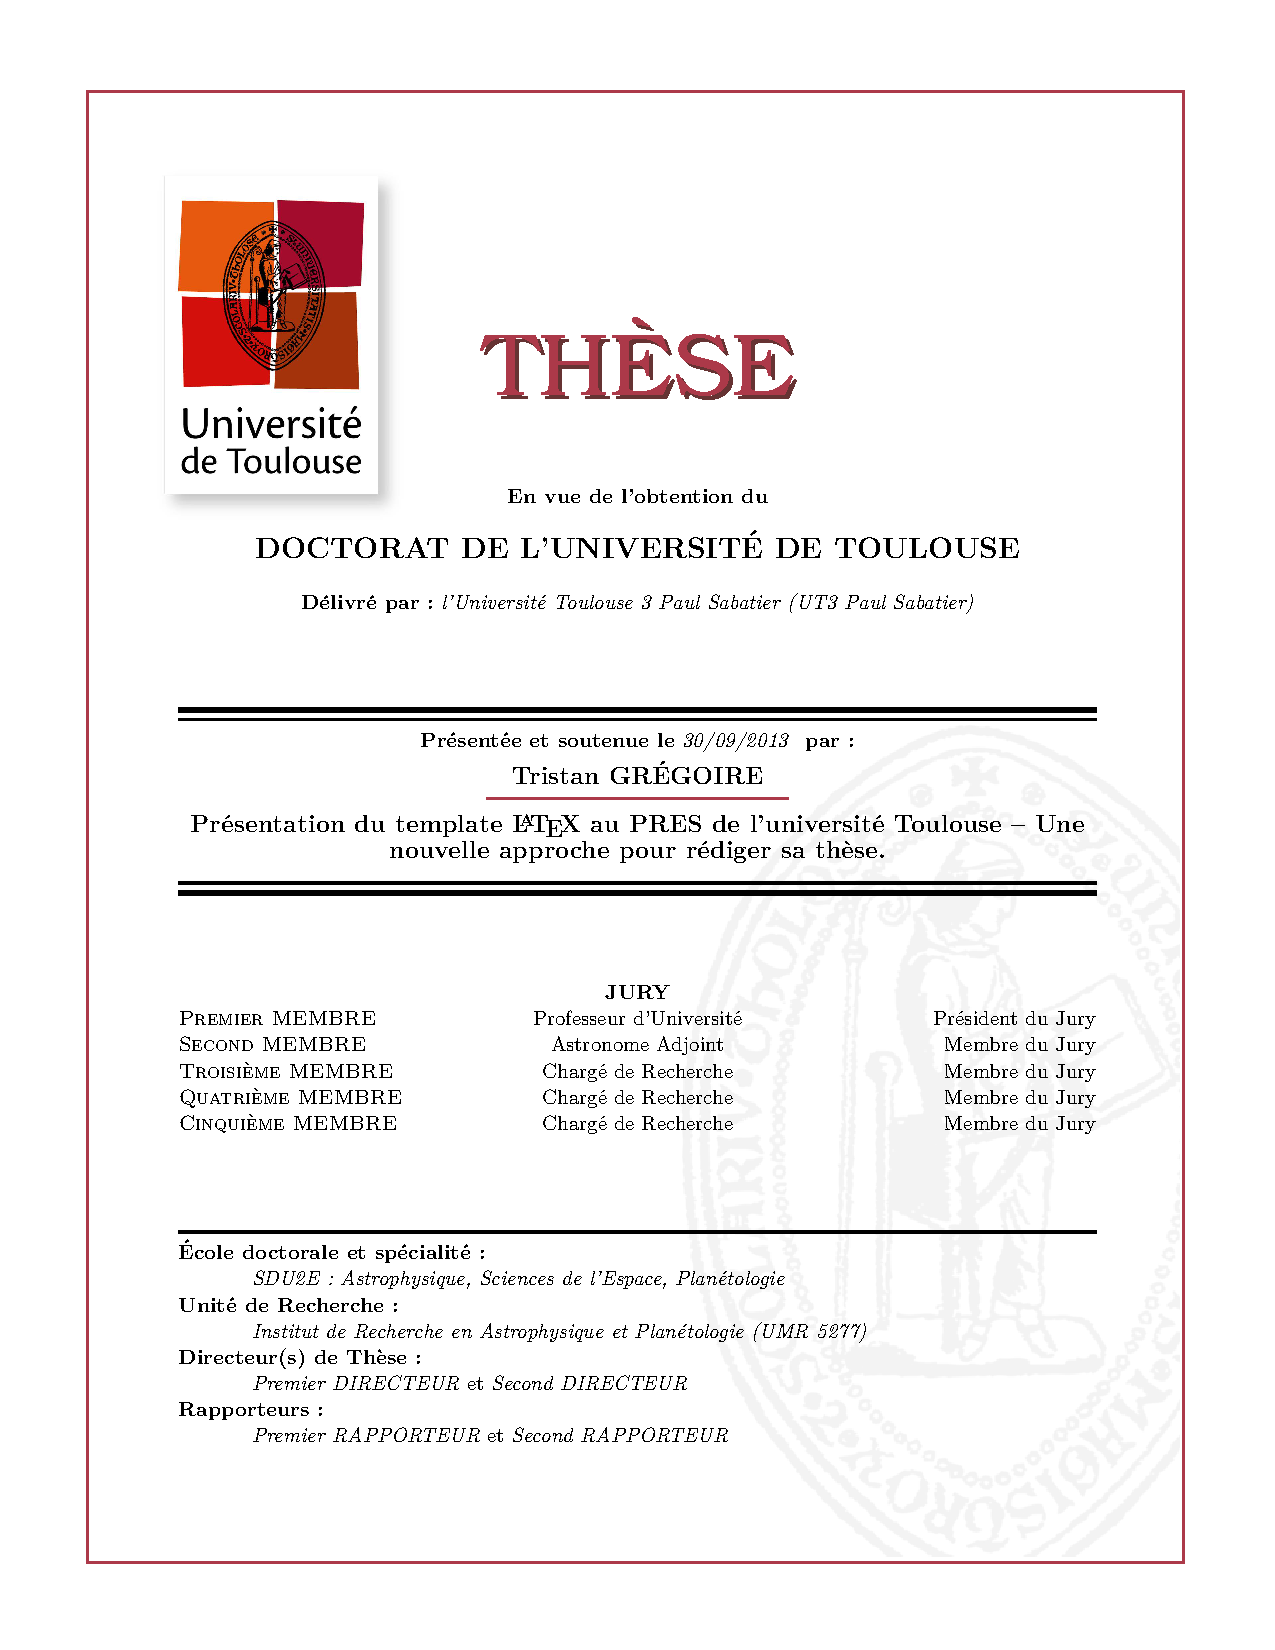
\includegraphics[width=\textwidth]{example-fr.pdf}
    \caption{\label{fig:ex}
        Rendu pour le code \LaTeX{} de \file{example-fr.tex} (pr\'esent\'e \`a la section~\ref{sec:ex}).
    }
\end{figure}
Le rendu de ce code est montr\'e dans la figure~\ref{fig:ex}.

%%%%%%%%%%%%%%%%%%%%%%
\newpage
\section*{Appendix}
\addcontentsline{toc}{section}{Appendix}
%%%%%%%%%%%%%%%%%%%%%%
\subsection{Ets-list\label{ssec:Ets}}
Liste compl\`ete des valeurs accept\'ees par l'option \texttt{Ets} sous la forme :
\texttt{OptionValue -> \'Etablissement}.
\lstinputlisting[firstline=5]{ETS-list.txt}
\subsection{ED-list\label{ssec:ED}}
Liste compl\`ete des valeurs accept\'ees par l'option \texttt{ED} sous la forme :
\texttt{OptionValue -> \'Ecole doctorale : Sp\'ecialit\'e}.
\lstinputlisting[firstline=5]{ED-list.txt}

%%%%%%%%%%%%%%%%%%%%%%
\section*{Remerciements}
\addcontentsline{toc}{section}{Remerciements}
%%%%%%%%%%%%%%%%%%%%%%
Remerciements particuliers \`a Bastien et Simon pour leurs id\'ees, commentaires et aides.

\noindent Ce paquet a \'et\'e d\'evelopp\'e par \textbf{Tristan GR\'EGOIRE}.
Si vous avez une quelconque question, n'h\'esitez pas \`a me contacter \`a \mail{tlsflyleaf@onada.fr}.

\medskip
\noindent\smiley \hfill Profitez de votre th\`ese $\ddot\smile$. \hfill \smiley

\bigskip
\hfill \copyright{} Tristan GR\'EGOIRE, 2013

\end{document}
